% !TeX root = RJwrapper.tex
\title{New Tools for Performing Financial Analysis Within the ``Tidy''
Ecosystem}
\author{by Matt Dancho, Davis Vaughan}

\maketitle

\abstract{%
Financial analysis and data science in the R programming language have
followed separate paths resulting in two important systems: ``xts'' and
``tidyverse''. The advantage of the ``xts'' system is in the management
of time series financial data. The advantage of the ``tidyverse'' system
is in the ability to implement a set of packages that have a uniform
structure and data representation to incorporate within the data science
workflow. Because of the separation in development, the two systems are
difficult to use together limiting the full potential of financial
analysis within R. The \texttt{tidyquant} package solves this problem by
integrating several of the best financial analysis packages with the
``tidy'' ecosystem. The integration unlocks the data science workflow,
which enables modeling and scaling analyses in a ``tidy'' way.

Three usage cases are discussed to illustrate the benefits of
\texttt{tidyquant}. The first example uses the scaling capabilities to
provide an answer for how the financial market values risk versus
reward. The second example builds on the first by visualizing the
returns over time and illustrating how the \texttt{purrr} package can be
used to apply functions to data frames. The third example evaluates
methods to scale the performance analysis of multiple portfolios using
combinations of weighted asset blends. These examples only scratch the
surface of what is possible with \texttt{tidyquant}.
}

\section{Status of Financial Analysis Tools in
R}\label{status-of-financial-analysis-tools-in-r}

The R programming language has seen immense growth in both popularity
and tools over the past several years, primarily driven by the
open-source nature of the R language and innovation in the field of data
science. The sub-segment of financial analysis in R is no different.
\href{https://timelyportfolio.github.io/rCharts_time_series/history.html}{TimelyPortfolio}
maintains a timeline of the major advances in R time series graphics,
which highlights the inception of several of the most influential R
financial and time series packages. Several packages are worth
describing in more detail as these create much of the current foundation
of R in Finance.

\begin{figure}[htbp]
  \centering
  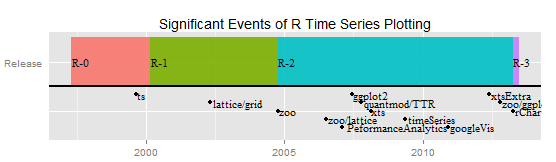
\includegraphics[width=13cm]{img/timeline}
  \timeline
\end{figure}

\subsection{quantmod / TTR}\label{quantmod-ttr}

The \emph{Quantitative Financial Modelling \& Trading Framework for R}
(\texttt{quantmod}) package and the \emph{Technical Trading Rules}
(\texttt{TTR}) package include mechanisms to retrieve, compute, and
visualize financial data using the most popular technical trading rules.

\subsection{xts / zoo}\label{xts-zoo}

The \emph{Extensible Time Series} (\texttt{xts}) package along with the
\texttt{zoo} package include mechanisms for the handling of time series
data. Most importantly, the \texttt{xts} package implemented a
cross-package method for handling the various time series data
structures, in the process solving a major shortcoming by managing
\emph{all major R time series objects}
\footnote{At least the following time series data objects exist in R to solve general and specific needs: `fts`, `its`, `irts`, `timeSeries`, `ti`, `ts`, `mts`, `zoo`, and `xts`. The sheer volume of options results in a complex decision process to determine which to use.}
under one class, \texttt{xts}.

\subsection{PerformanceAnalytics}\label{performanceanalytics}

The \texttt{PerformanceAnalytics} package includes a large collection of
econometric functions for financial performance analysis, many of which
are described in \emph{Practical Portfolio Performance Measurement and
Attribution} by Carl Bacon \citep{Bacon2004}. These functions enable
analysis of individual asset and portfolio (the weighted aggregation of
multiple assets) returns using popular statistical methods for measuring
performance.

\section{New Tools: tidyverse}\label{new-tools-tidyverse}

In parallel with the progression in the R in Finance community,
developers at \emph{RStudio} have been creating useful tools for data
science in R, namely the ``tidyverse''. The ``tidyverse'', or ``tidy''
ecosystem, is a collection of packages that fundamentally and
philosophically work together utilizing a common ``tidy'' data
representation, which is defined in \emph{Tidy Data} \citep{tidy-data}.
To summarize, the ``tidy'' data representation reserves \emph{each
variable as a column, each observation as a row, and each value as a
cell}.\footnote{The "tidy" data format is often referred to as "long" format versus "wide" format because the observations within the data set extend row-wise versus column-wise. }
The ``tidyverse'' packages all share a common API design and fit
together seamlessly within the data science workflow. Additionally, the
``tidyverse'' packages are documented in the online text, \emph{R for
Data Science} \citep{R4DS2017}, which is the de facto manual for data
scientists beginning with the R programming language. The ``tidyverse''
includes several packages worth describing in more detail.

\begin{figure}[htbp]
  \centering
  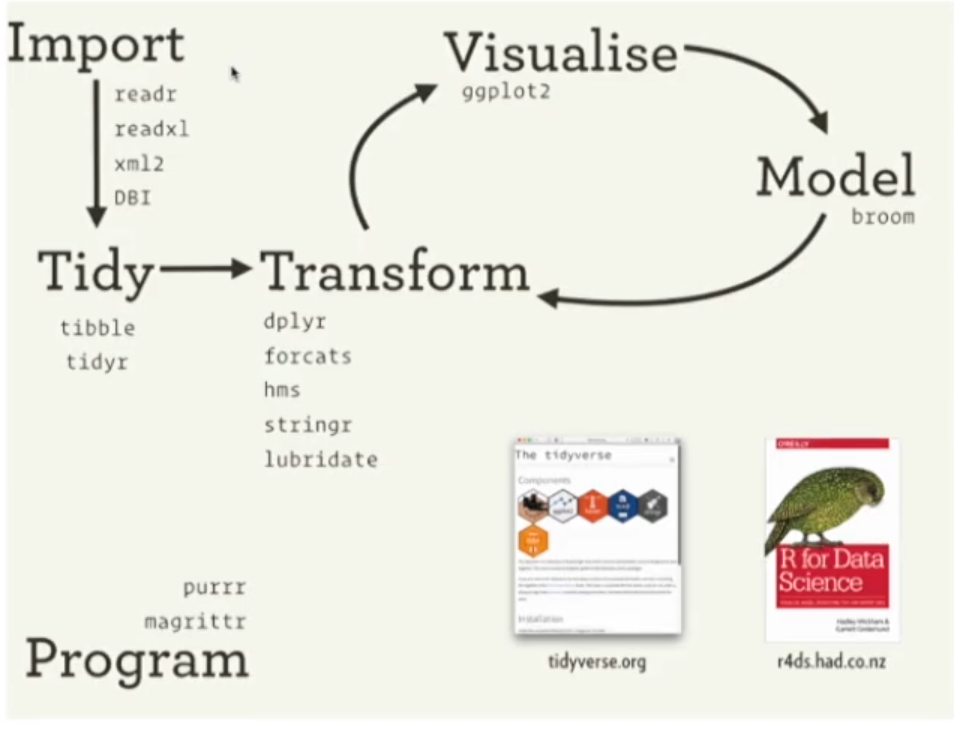
\includegraphics[width=12cm, height=8cm]{img/tidyverse}
  \tidyverse
\end{figure}

\subsection{dplyr / tidyr}\label{dplyr-tidyr}

The \texttt{dplyr} and \texttt{tidyr} packages provide tools to clean
and manipulate data. Historically, the \texttt{plyr} package, the
precursor to \texttt{dplyr}, was developed as a mechanism to implement
the \emph{split-apply-combine} framework popularized by Hadley Wickham
in \emph{The Split-Apply-Combine Strategy for Data Analysis}
\citep{plyr}. The \texttt{dplyr} package advanced this concept by
implementing this framework internally along with providing many
additional tools that work naturally within the framework. The
\texttt{tidyr} package enables users to format the data in a ``tidy''
way. The major advances were threefold. First, the packages simplified
and made consistent many of the most common data manipulation and
summarization tasks in R. Second, the packages implement the
\emph{split-apply-combine} framework internally allowing users to work
with grouped and nested data sets. Third, the packages incorporated the
use of the pipe (\texttt{\%\textgreater{}\%}) from the \texttt{magrittr}
package enabling functional verbs to follow an easy, efficient, and
human-readable workflow.

\subsection{purrr}\label{purrr}

The \texttt{purrr} package provides tools for applying functions to data
frames. Similar to the traditional \texttt{apply} function in base R,
the \texttt{map} function enables ``mapping'' functions row-wise within
a data frame. The major advance is the ability to scale analysis. An
analysis can be performed with ``nested'' data frames allowing users to
apply functions across many independent data sets, a common task in data
science. Further, the resulting data frame is ``tidy'', each analysis
result is kept alongside the data that generated it.

\subsection{tibble}\label{tibble}

The \texttt{tibble} package extends the traditional \texttt{data.frame}
object by providing useful tools for creating and coercing objects to
``tibbles'' or ``tidy'' data frames.

\subsection{ggplot2}\label{ggplot2}

The \texttt{ggplot2} package provides mechanisms for creating complex
visualizations using a layered approach called the ``grammar of
graphics'', which is discussed in \emph{A Layered Grammar of Graphics}
\citep{layered-grammar}. The \texttt{ggplot2} package is the primary
package for creating static graphics in the ``tidy'' ecosystem.

\subsection{lubridate}\label{lubridate}

The \texttt{lubridate} package includes functions to manage date and
date-time objects in R, which is discussed in \emph{Dates and Times Made
Easy with lubridate} \citep{lubridate}. The combination of
\texttt{lubridate} with \texttt{dplyr} enables easy coercion of
character class to date and date-time, filtering and subsetting on
dates, and many more complex tasks that are essential to financial
analysis. Further, combining \texttt{lubridate} with \texttt{ggplot2}
enables graphical visualization using dates and date-times.

\section{Different Data Structures, Each with
Advantages}\label{different-data-structures-each-with-advantages}

All of the major financial packages work within the ``xts'' system,
which is specifically designed for time series analysis. The system
works very well. The extensible time series, ``xts'', data structure is
similar to a numeric ``matrix''. The primary difference is that row
names consist of the date or date-time information. The objects can be
subset by date or transformed to different periodicity very easily using
a wide variety of flexible functions built to operate within the ``xts''
time-based system. Because of its focus, flexibility and design, the
``xts'' system manages single assets of the numeric time-based data
extremely well. Multiple assets are handled by merging columns for
different groups in a ``wide'' format, which is different than the
``tidy'' data representation (i.e. ``long'' format). The system has been
designed to manage this data representation.

Much of the recent innovation in data science has occurred within the
``tidy'' ecosystem. With the entrance of the ``tidyverse'', grouping and
iteratively applying functions (i.e.~scaling analysis) has become easy,
efficient, and a core principle. Further, advances in date and date-time
functionality have enabled management of time series data within the
``tibble'' data structure. As the data science field grows, more
innovative functionality will be developed within the ``tidy''
ecosystem, much of which will be (and is already) useful to the field of
financial analysis.

The two systems have advantages that are needed within the realm of
financial analysis. The ``xts'' system has the infrastructure to perform
financial analytics. The ``tidyverse'' has the functions and data
representation to seamlessly scale analysis using the data science
workflow. Unfortunately, the two systems do not work well together. The
``xts'' system has underlying dependencies on the ``matrix'' data
structure whereas the ``tidy'' ecosystem is built on top of the
``tibble'' (``tidy'' data frame) data structure. The ``matrix''
structure is \emph{homogenous}, the entire matrix must hold the same
data type. In R, coercion rules take over when data types are combined
within a ``matrix''. For example, combining a character and a numeric
class will result in a character only matrix. As a result, the ``xts''
system can not be formatted in a ``tidy'' structure with each variable
as a column, each observation as a row, and each value in a cell. The
solution is to merge data sets together keeping the column names as the
observation. This works well in the ``xts'' system, but presents
problems in the ``tidyverse'' system since the data is not represented
following the ``tidy'' principles. Conversely, the ``tibble'' structure
is \emph{heterogenous}, each column can contain a different data type.
This works extremely well for grouping observations together. For
example, a ``tibble'' can contain symbols in one column and daily prices
in another column. This enables applying functions to groups
(e.g.~symbol) for scaling analyses. The end result is two excellent
systems that do not communicate easily. Without communication between
systems, the full potential of financial analysis within R is limited.

To solve this problem, the \texttt{tidyquant} package was developed to
integrate many of the ``xts'' based financial analysis packages into the
``tidyverse''. The central motivation behind the integration is to
enable the user to gain the benefits of both systems. The
\texttt{tidyquant} package works with ``tidy'' input and output, fitting
seamlessly within the ``tidy'' ecosystem allowing for analysis to follow
the data science workflow discussed in detail in \emph{R for Data
Science} \citep{R4DS2017}. Internally, \texttt{tidyquant} leverages the
``xts'' system as the engine to perform financial computations. This
enables almost all of the functionality of \texttt{quantmod},
\texttt{TTR}, \texttt{PerformanceAnalytics}, \texttt{xts} and
\texttt{zoo} to be used integrally (without switching back and forth)
within the ``tidy'' ecosystem.

In the next section, an analysis is performed with the ``tidyverse'' to
illustrate the benefits in manipulating grouped financial data. Then, in
the final section, a demonstration of the \texttt{tidyquant} package is
performed to illustrate some of its key benefits within the realm of
financial analysis.

\section{\texorpdfstring{Benefits of the
``tidyverse''}{Benefits of the tidyverse}}\label{benefits-of-the-tidyverse}

One of the primary benefits of the ``tidyverse'' is the ability to work
with grouped data sets. The core concept is to split a data set into
groups, apply functions to independent groups, then recombine the
results. The value in this approach is the ability to scale analyses
from one group to many groups and then compare the results. A simple
example using the \texttt{FANG} data set from the \texttt{tidyquant}
package illustrates this framework.

Start with a question: \emph{What is the historical performance for the
FANG tech stocks?}

Load the ``tidyverse'' libraries. The \texttt{tidyquant} package is
loaded to get the \texttt{FANG} data set and to load the
\texttt{tidyverse} package. Only \texttt{tidyverse} functionality will
be used in this example.

\begin{Schunk}
\begin{Sinput}
library(tidyquant) 
data("FANG")       
\end{Sinput}
\end{Schunk}

Next, view the data set. The data consists of the historical daily stock
prices for the
``FANG''\footnote{The acronym, "FANG", was popularized by Jim Cramer of the popular CNBC show, Mad Money. http://www.investopedia.com/terms/f/fang-stocks-fb-amzn.asp.}
tech stocks (``FB'', ``AMZN'', ``NFLX'', and ``GOOG'') spanning from the
beginning of 2013 to the end of 2016.

\begin{Schunk}
\begin{Sinput}
head(FANG)
dim(FANG)
\end{Sinput}
\end{Schunk}

\begin{tabular}{cccccccc}
\toprule
symbol & date & open & high & low & close & volume & adjusted\\
\midrule
FB & 2013-01-02 & 27.44 & 28.18 & 27.42 & 28.00 & 69846400 & 28.00\\
FB & 2013-01-03 & 27.88 & 28.47 & 27.59 & 27.77 & 63140600 & 27.77\\
FB & 2013-01-04 & 28.01 & 28.93 & 27.83 & 28.76 & 72715400 & 28.76\\
FB & 2013-01-07 & 28.69 & 29.79 & 28.65 & 29.42 & 83781800 & 29.42\\
FB & 2013-01-08 & 29.51 & 29.60 & 28.86 & 29.06 & 45871300 & 29.06\\
FB & 2013-01-09 & 29.67 & 30.60 & 29.49 & 30.59 & 104787700 & 30.59\\
\bottomrule
\end{tabular}

{[}1{]} 4032 8

\hspace{20 mm}

Historical performance is a function of the period returns
(i.e.~percentage change between current price and previous price). A
wealth index is often used to assess the investment growth, which is the
product of the period returns and asset value during the previous
period. The data workflow is split into two steps.

\begin{enumerate}
\def\labelenumi{\arabic{enumi}.}
\tightlist
\item
  Calculate the period returns
\item
  Calculate the cumulative performance using a wealth index
\end{enumerate}

Calculate the period returns. A lag is needed to line up the previous
period return with the current period return. The difference is then
taken, and from the difference the period return is calculated as the
percentage change from the initial value.

For a more granular look at the code, each of the functions do the
following. Only the ``symbol'', ``date'' and ``adjusted'' price columns
are needed to start, so a \texttt{select} statement removes the
unnecessary columns. Then, the data is grouped by ``symbol'' using the
\texttt{group\_by} function. The \texttt{mutate} function adds
calculated columns to a data frame. The ``lag'' is calculated using the
\texttt{lag} function from \texttt{dplyr}. The ``diff'' is the
``adjusted'' closing price minus the ``lag''. The ``period.returns'' is
the percentage change from the ``adjusted'', which is ``diff'' divided
by ``adjusted''. The \texttt{replace\_na} function is used to switch
\texttt{NA} values with zero. Note that an ungrouped ``tibble'' is
returned due to the \texttt{replace\_na} function.

\begin{Schunk}
\begin{Sinput}
FANG_returns <- FANG %>%
    select(-(open:volume)) %>%
    group_by(symbol) %>%
    mutate(lag = lag(adjusted),
           diff = adjusted - lag,
           period.returns = diff / adjusted) %>%
    replace_na(list(period.returns = 0)) 
head(FANG_returns)
dim(FANG_returns)
\end{Sinput}
\end{Schunk}

\begin{tabular}{cccccc}
\toprule
symbol & date & adjusted & lag & diff & period.returns\\
\midrule
FB & 2013-01-02 & 28.00 & NA & NA & 0.0000000\\
FB & 2013-01-03 & 27.77 & 28.00 & -0.230000 & -0.0082823\\
FB & 2013-01-04 & 28.76 & 27.77 & 0.990000 & 0.0344228\\
FB & 2013-01-07 & 29.42 & 28.76 & 0.660000 & 0.0224337\\
FB & 2013-01-08 & 29.06 & 29.42 & -0.360001 & -0.0123882\\
FB & 2013-01-09 & 30.59 & 29.06 & 1.530001 & 0.0500164\\
\bottomrule
\end{tabular}

{[}1{]} 4032 6

\hspace{20 mm}

Now, the wealth index can be calculated. The wealth index is the
cumulative product of the period returns multiplied by the initial
investment value. An initial investment of \$10K USD is used as an
example.

\begin{Schunk}
\begin{Sinput}
initial_investment <- 10000
FANG_performance <- FANG_returns %>%
    group_by(symbol) %>%
    mutate(wealth.index = initial_investment * cumprod(1 + period.returns)) 
head(FANG_performance)
dim(FANG_performance)
\end{Sinput}
\end{Schunk}

\begin{tabular}{ccccccc}
\toprule
symbol & date & adjusted & lag & diff & period.returns & wealth.index\\
\midrule
FB & 2013-01-02 & 28.00 & NA & NA & 0.0000000 & 10000.000\\
FB & 2013-01-03 & 27.77 & 28.00 & -0.230000 & -0.0082823 & 9917.177\\
FB & 2013-01-04 & 28.76 & 27.77 & 0.990000 & 0.0344228 & 10258.554\\
FB & 2013-01-07 & 29.42 & 28.76 & 0.660000 & 0.0224337 & 10488.691\\
FB & 2013-01-08 & 29.06 & 29.42 & -0.360001 & -0.0123882 & 10358.755\\
FB & 2013-01-09 & 30.59 & 29.06 & 1.530001 & 0.0500164 & 10876.863\\
\bottomrule
\end{tabular}

{[}1{]} 4032 7

\hspace{20 mm}

Lastly, the performance of the individual stocks using daily compounding
of the returns are visualized using \texttt{ggplot2}.

\begin{Schunk}
\begin{Sinput}
FANG_performance %>%
    ggplot(aes(x = date, y = wealth.index, color = symbol)) +
    geom_line() +
    labs(title = "Individual Stocks: Comparing the Growth of 10K",
         x = "", y = "Investment Value") +
    scale_y_continuous(labels = scales::dollar) + 
    theme_minimal()
\end{Sinput}


\begin{center}\includegraphics{RInFinanceRticles_files/figure-latex/unnamed-chunk-9-1} \end{center}

\end{Schunk}

The ``tidy'' ecosystem can be used to solve a wide range of complex
problems because it enables grouping of data sets and applying a data
science workflow. In the next section, examples are presented to
illustrate the power of combining the financial analysis tools from the
``xts'' system with the ``tidyverse'' for financial applications.

\section{\texorpdfstring{Financial Applications with
``tidyquant''}{Financial Applications with tidyquant}}\label{financial-applications-with-tidyquant}

The financial analysis packages are difficult or impossible to use
within the ``tidy'' ecosystem. A new tool is needed, \texttt{tidyquant}.
The \texttt{tidyquant} package has one major advantage: it integrates
the ``xts'' based financial packages with the ``tidyverse'' to enable
the data science workflow and ``tidy'' ecosystem functionality to be
applied to financial analysis. The innovation is relatively minor on a
conceptual level, but the net effect is significant in that the tools
within the ``tidy'' ecosystem are now unlocked for financial analysis.
The following examples illustrate the new capability.

\subsection{Example 1: Evaluating Risk vs
Reward}\label{example-1-evaluating-risk-vs-reward}

Financial analysis is almost always a trade off between risk and reward.
Reward is measured by the growth of an investment. Risk is typically
associated with volatility. Often when beginning an analysis, one wishes
to understand the components of a market basket of stocks on the basis
of this risk-reward trade off in order to screen investments.

Start with a question: \emph{How does the market value risk versus
reward?}

This question is answerable by comparing the risk and reward
characteristics for a basket of stocks viewed as a reasonable proxy for
the ``market''. The observations within the market are stocks. Stocks
also have observations, or historical prices, which can be obtained over
time and can be used to evaluate various statistical qualities that
relate to risk versus reward. The reward is the return performance
(i.e.~returns), which is the positive or negative percentage change
between observations. When accumulated across a frequency such as daily,
the large set of returns has statistical properties that can be
measured. To simplify the question, the average and standard deviation
of the returns can be used as a general proxy of risk versus reward.
When pooled together, the stocks can thus be compared to expose general
performance trends within the market.
\footnote{Using the mean and standard deviation of stock returns has roots in Brownian motion, known as a Stochastic Process, which is often used in Monte Carlo simulation to predict the range of future returns within a confidence interval based on the properties of past returns. }

To start, load \texttt{tidyquant}, which loads all of the packages
needed to evaluate risk versus reward.

\begin{Schunk}
\begin{Sinput}
# Loads tidyquant, tidyverse, lubridate, quantmod, TTR, xts, zoo, PerformanceAnalytics
library(tidyquant)
\end{Sinput}
\end{Schunk}

Next, collect ticker data. The question implies that a large sample of
stock data is needed to evaluate how performance and risk is valued
within the market. The S\&P 500 index is a good place to start.
\texttt{tidyquant} includes a function, \texttt{tq\_index}, which
returns the stock symbols and company names for every stock within an
index.

\begin{Schunk}
\begin{Sinput}
sp500 <- tq_index("SP500")
head(sp500)
dim(sp500)
\end{Sinput}
\end{Schunk}

\begin{tabular}{cc}
\toprule
symbol & company\\
\midrule
MMM & 3M\\
ABT & ABBOTT LABORATORIES\\
ABBV & ABBVIE INC\\
ACN & ACCENTURE\\
ATVI & ACTIVISION BLIZZARD\\
AYI & ACUITY BRANDS\\
\bottomrule
\end{tabular}

{[}1{]} 502 2

\hspace{20 mm}

Next, the historical stock prices are needed for each stock within the
S\&P 500 index. The stock prices are easy to retrieve at scale using the
function, \texttt{tq\_get}, with the ``get'' option,
\texttt{get\ =\ "stock.prices"}. \texttt{tq\_get} is a wrapper for
\texttt{quantmod::getSymbols}, which enables passing the underlying
function parameters \texttt{from} and \texttt{to}. The input to
\texttt{tq\_get} is \texttt{data}, which can be a single stock symbol, a
vector of stock symbols, or a tibble with stock symbols in the first
column. The latter is passed to \texttt{tq\_get} using the pipe
(\texttt{\%\textgreater{}\%}). The function may take a few minutes to
run because it is downloading the past ten years of daily open, high,
low, close, volume, and adjusted stock prices for the entire S\&P 500
index into one ``tidy'' data frame. Reviewing the results indicates that
the prices were retrieved in entirety. The resulting ``tibble'' has
1,205,845 rows and 502 unique symbols.

\begin{Schunk}
\begin{Sinput}
sp500_stock_prices <- sp500 %>%
    tq_get(get  = "stock.prices", 
           from = "2007-01-01", 
           to   = "2017-01-01")
head(sp500_stock_prices)
dim(sp500_stock_prices)
\end{Sinput}
\end{Schunk}

\begin{tabular}{ccccccccc}
\toprule
symbol & company & date & open & high & low & close & volume & adjusted\\
\midrule
MMM & 3M & 2007-01-03 & 77.53 & 78.85 & 77.38 & 78.26 & 3781500 & 60.31064\\
MMM & 3M & 2007-01-04 & 78.40 & 78.41 & 77.45 & 77.95 & 2968400 & 60.07174\\
MMM & 3M & 2007-01-05 & 77.89 & 77.90 & 77.01 & 77.42 & 2765200 & 59.66330\\
MMM & 3M & 2007-01-08 & 77.42 & 78.04 & 76.97 & 77.59 & 2434500 & 59.79431\\
MMM & 3M & 2007-01-09 & 78.00 & 78.23 & 77.44 & 77.68 & 1896800 & 59.86367\\
MMM & 3M & 2007-01-10 & 77.31 & 77.96 & 77.04 & 77.85 & 1787500 & 59.99468\\
\bottomrule
\end{tabular}

{[}1{]} 1205845 9

\hspace{20 mm}

Next, the prices are grouped by stock symbol to calculate the
logarithmic daily returns for each stock. The transform is applied using
\texttt{tq\_transmute}, which is used in situations where periodicity
changes (or can change). The \texttt{quantmod} OHLC (open, high, low,
close) notation is used to collect the adjusted prices
(\texttt{ohlc\_fun\ =\ Ad}) and send these prices to the
\texttt{periodReturn} function (\texttt{mutate\_fun\ =\ periodReturn}).
The additional arguments \texttt{period\ =\ "daily"} and
\texttt{type\ =\ "log"} are passed to the mutating function,
\texttt{periodReturn}. The daily log returns (DLR) for each of the 502
groups of stock symbols is generated below.

\begin{Schunk}
\begin{Sinput}
sp500_returns <- sp500_stock_prices %>%
    group_by(symbol) %>%
    tq_transmute(ohlc_fun = Ad, mutate_fun = periodReturn, 
                 period = "daily", type = "log", col_rename = "dlr")
head(sp500_returns)
dim(sp500_returns)
\end{Sinput}
\end{Schunk}

\begin{tabular}{ccc}
\toprule
symbol & date & dlr\\
\midrule
MMM & 2007-01-03 & 0.0000000\\
MMM & 2007-01-04 & -0.0039691\\
MMM & 2007-01-05 & -0.0068224\\
MMM & 2007-01-08 & 0.0021934\\
MMM & 2007-01-09 & 0.0011593\\
MMM & 2007-01-10 & 0.0021860\\
\bottomrule
\end{tabular}

{[}1{]} 1205845 3

\hspace{20 mm}

Next, the mean and standard deviation of the daily log returns are used
to evaluate and compare the stocks. The easiest way is to use
\texttt{tq\_performance}, which applies the
\texttt{PerformanceAnalytics} performance functions to ``tidy'' data
frames of asset or portfolio returns. The \texttt{table.Stats} function
returns the arithmetic mean and standard deviation along with a number
of other useful statistics that characterize the returns.

\begin{Schunk}
\begin{Sinput}
sp500_stats <- sp500_returns %>%
    tq_performance(Ra = dlr, performance_fun = table.Stats, ci = 0.95, digits = 6) 
sp500_stats %>%
    select(1:5) %>%
    head()
dim(sp500_stats)
\end{Sinput}
\end{Schunk}

\begin{tabular}{ccccc}
\toprule
symbol & ArithmeticMean & GeometricMean & Kurtosis & LCLMean(0.95)\\
\midrule
MMM & 0.000431 & 0.000331 & 5.806040 & -0.000120\\
ABT & 0.000302 & 0.000215 & 6.294066 & -0.000211\\
ABBV & 0.000714 & 0.000565 & 3.868658 & -0.000350\\
ACN & 0.000543 & 0.000404 & 8.532566 & -0.000108\\
ATVI & 0.000604 & 0.000359 & 10.735599 & -0.000263\\
AYI & 0.000701 & 0.000420 & 6.011008 & -0.000225\\
\bottomrule
\end{tabular}

{[}1{]} 502 17

\hspace{20 mm}

The data required to visualize risk versus reward is complete. A plot of
the mean daily log returns (MDLR) versus the standard deviation of daily
log returns (SDDLR) shows the relationship. Note that observations
(stocks) with fewer than five years of trading days (5 years x 252 trade
days per year) are removed from the visualization to yield a long-run
perspective.

\begin{Schunk}
\begin{Sinput}
sp500_stats %>%
    filter(Observations >= 252 * 5) %>%
    ggplot(aes(x = Stdev, y = ArithmeticMean)) +
    geom_point(alpha = 0.5, col = "steelblue") +
    geom_smooth(method = "lm") +
    labs(title = "Evaluating Risk Vs Reward for Stocks in the SP500",
         subtitle = "An inverse trend between volatility (SDDLR) and returns (MDLR)",
         x = "Standard Deviation of Daily Log Returns (SDDLR)",
         y = "Arithmetic Mean of Daily Log Returns (MDLR)") +
    theme_tq()
\end{Sinput}


\begin{center}\includegraphics{RInFinanceRticles_files/figure-latex/unnamed-chunk-19-1} \end{center}

\end{Schunk}

By comparing an entire basket of stocks, reasonable trading strategies
can be developed. For example, creating a portfolio that minimizes
volatility may result in higher performance over the long run. This is
easily seen in the trend line indicating an inverse trend between
volatility (SDDLR) and returns (MDLR). Further, once trading strategies
are developed, screening is easily implemented by filtering the data
set.

\begin{Schunk}
\begin{Sinput}
sp500_high_performers <- sp500_stats %>%
    filter(Observations >= 252 * 5,
           Stdev <= 0.02,
           ArithmeticMean >= 0.0005) %>%
    arrange(desc(ArithmeticMean)) 
sp500_high_performers %>%
    select(1:5) %>%
    head()
\end{Sinput}
\end{Schunk}

\begin{tabular}{ccccc}
\toprule
symbol & ArithmeticMean & GeometricMean & Kurtosis & LCLMean(0.95)\\
\midrule
TDG & 0.00116 & 0.00097 & 7.96994 & 0.00039\\
FBHS & 0.00111 & 0.00094 & 2.58643 & 0.00011\\
DLPH & 0.00094 & 0.00079 & 4.21629 & 0.00000\\
ROST & 0.00090 & 0.00073 & 5.15896 & 0.00019\\
ORLY & 0.00086 & 0.00070 & 10.20942 & 0.00016\\
AGN & 0.00082 & 0.00067 & 6.06114 & 0.00013\\
\bottomrule
\end{tabular}

{[}1{]} 52 17

\hspace{20 mm}

\subsection{\texorpdfstring{Example 2: Visualizing Return Consistency
Among ``High
Performers''}{Example 2: Visualizing Return Consistency Among High Performers}}\label{example-2-visualizing-return-consistency-among-high-performers}

Example 1 can be expanded upon using the notion that excessive
volatility is a factor that the market tends to penalize. In this
example, the goal is to visualize returns of the top ranked prospects
from Example 1 to determine if the stock is consistently growing. This
example will introduce a new package called \texttt{purrr}, which is
used to map functions to ``nested'' data frames.

Start with a question: \emph{Of the best stocks from Example 1, which
offer the most consistent growth?}

The easiest way to answer this question is to visualize the mean daily
log returns (MDLR) by year. Collecting the means by year can be
accomplished in a number of ways. The \texttt{purrr} package offers a
new approach by mapping functions to tibble groups similar to the
\texttt{apply} function in base R. The nice thing about \texttt{map} is
that if a function can be applied to one group of the data, it can be
``mapped'' to many groups. This example will proceed as follows:

\begin{enumerate}
\def\labelenumi{\arabic{enumi}.}
\tightlist
\item
  Retrieve the symbols of the top \emph{n} performers. The example uses
  the top 10, but any number can be selected.
\item
  Filter and ``nest'' the returns for the top performers.
\item
  Create a custom function to map to each of the nested ``tibbles''.
\item
  Map the custom function to the ``tibble''.
\item
  Unnest the data frame.
\item
  Visualize the results.
\end{enumerate}

First, get the symbols of the top performers. Since the
\texttt{sp\_500\_high\_performers} data frame is arranged in decreasing
MDLR, the \texttt{slice} function can be used to collect the top
performers.

\begin{Schunk}
\begin{Sinput}
n <- 10
high_performers <- sp500_high_performers %>%
    ungroup() %>%
    select(symbol, ArithmeticMean, Stdev) %>%
    slice(1:n)
high_performers
\end{Sinput}
\end{Schunk}

\begin{tabular}{ccc}
\toprule
symbol & ArithmeticMean & Stdev\\
\midrule
TDG & 0.001157 & 0.019580\\
FBHS & 0.001110 & 0.018597\\
DLPH & 0.000938 & 0.017123\\
ROST & 0.000897 & 0.018166\\
ORLY & 0.000857 & 0.017784\\
\addlinespace
AGN & 0.000825 & 0.017793\\
EW & 0.000817 & 0.019710\\
DLTR & 0.000803 & 0.019179\\
AZO & 0.000753 & 0.015612\\
TJX & 0.000708 & 0.017008\\
\bottomrule
\end{tabular}

\hspace{20 mm}

Next, filter the S\&P 500 returns tibble to only the stocks of interest
and ``nest'' the tibble. Nesting works on groups, so all of the data
that is grouped on gets wrapped up into a list column.

\begin{Schunk}
\begin{Sinput}
high_performer_returns_nested <- sp500_returns %>%
    filter(symbol %in% high_performers$symbol) %>%
    nest()
high_performer_returns_nested
\end{Sinput}
\begin{Soutput}
#> # A tibble: 10 × 2
#>    symbol                 data
#>     <chr>               <list>
#> 1     AGN <tibble [2,518 × 2]>
#> 2     AZO <tibble [2,518 × 2]>
#> 3    DLPH <tibble [1,288 × 2]>
#> 4    DLTR <tibble [2,518 × 2]>
#> 5      EW <tibble [2,518 × 2]>
#> 6    FBHS <tibble [1,332 × 2]>
#> 7    ORLY <tibble [2,518 × 2]>
#> 8    ROST <tibble [2,518 × 2]>
#> 9     TJX <tibble [2,518 × 2]>
#> 10    TDG <tibble [2,518 × 2]>
\end{Soutput}
\end{Schunk}

\hspace{20 mm}

Once the tibble is nested, create a custom function to apply to each of
the nested tibbles. The function \texttt{calculate\_mdlr\_by\_year}
transforms the daily log returns to mean daily log returns by year.

\begin{Schunk}
\begin{Sinput}
calculate_mdlr_by_year <- function(dlr) {
    dlr %>%
        mutate(year = year(date)) %>%
        group_by(year) %>%
        summarize(mdlr.by.year = mean(dlr))
}
\end{Sinput}
\end{Schunk}

Map the custom function, \texttt{calculate\_mdlr\_by\_year}, to the
nested data frame. This is done using \texttt{mutate} with \texttt{map}.
The ``data'' column is no longer needed, so it is removed with
\texttt{select}.

\pagebreak

\begin{Schunk}
\begin{Sinput}
high_performer_returns_mapped <- high_performer_returns_nested %>%
    mutate(mdlr.by.year = map(data, calculate_mdlr_by_year)) %>%
    select(-data)
high_performer_returns_mapped
\end{Sinput}
\begin{Soutput}
#> # A tibble: 10 × 2
#>    symbol      mdlr.by.year
#>     <chr>            <list>
#> 1     AGN <tibble [10 × 2]>
#> 2     AZO <tibble [10 × 2]>
#> 3    DLPH  <tibble [6 × 2]>
#> 4    DLTR <tibble [10 × 2]>
#> 5      EW <tibble [10 × 2]>
#> 6    FBHS  <tibble [6 × 2]>
#> 7    ORLY <tibble [10 × 2]>
#> 8    ROST <tibble [10 × 2]>
#> 9     TJX <tibble [10 × 2]>
#> 10    TDG <tibble [10 × 2]>
\end{Soutput}
\end{Schunk}

Now, \texttt{unnest} the ``mdlr.by.year'' column to return the MDLR by
year for each of the high performing stocks.

\begin{Schunk}
\begin{Sinput}
high_performer_returns_mapped %>%
    unnest() %>%
    head()
\end{Sinput}
\end{Schunk}

\begin{tabular}{ccc}
\toprule
symbol & year & mdlr.by.year\\
\midrule
AGN & 2007 & 0.0001253\\
AGN & 2008 & -0.0000839\\
AGN & 2009 & 0.0015845\\
AGN & 2010 & 0.0010532\\
AGN & 2011 & 0.0006171\\
AGN & 2012 & 0.0014174\\
\bottomrule
\end{tabular}

\hspace{20 mm}

Finally, visualize the results using \texttt{ggplot2}. The mean daily
log returns when averaged by year yields a different picture then what
the results of Example 1 portrayed. Some of the stocks exhibit
consistent growth (e.g.~ROST) while others have more volatile returns or
negative returns in multiple years indicating a lack of consistency
(e.g.~DLPH).

\begin{Schunk}
\begin{Sinput}
high_performer_returns_mapped %>%
    unnest() %>%
    ggplot(aes(x = year, y = mdlr.by.year, color = symbol)) +
    geom_hline(yintercept = 0, color = palette_light()[[1]]) +
    geom_line(size = 1) +
    geom_point(size = 2) +
    geom_smooth(method = "lm", se = FALSE, color = "blue") +
    scale_color_tq() +
    theme_tq() +
    facet_wrap(~ symbol, ncol = 5) +
    labs(title = "Comparing the Consistency of High Performers",
         y = "Mean Daily Log Returns (MDLR)", color = "") +
    theme(axis.text.x = element_text(angle = 60, hjust = 1),
          axis.title.x = element_blank())
\end{Sinput}


\begin{center}\includegraphics{RInFinanceRticles_files/figure-latex/unnamed-chunk-29-1} \end{center}

\end{Schunk}

\hspace{20 mm}

This analysis can be expanded even further. With the data science
modeling workflow discussed in \emph{R for Data Science}
\citep{R4DS2017}, a financial analyst or engineer can apply prediction
models to the data set (refer to the chapters on modeling using the
\texttt{broom} package). Custom screening metrics can be developed such
as using the coefficients of a regression model, counting the times an
investment falls below zero, calculating standard deviation in MDLR by
year, and more. Screening investments within an entire index or exchange
becomes relatively easy, even with complex metrics. The blog article,
\emph{Russell 2000 Quantitative Stock Analysis in R: Six Stocks with
Amazing, Consistent Growth} \citep{russell2000}, elaborates on the
details behind using the \texttt{purrr} package to create complex
screening metrics.

\subsection{Example 3: Evaluating Performance of Multiple Portfolio
Blends}\label{example-3-evaluating-performance-of-multiple-portfolio-blends}

Portfolio aggregation (the aggregation of assets using a weighted blend)
is a useful technique to reduce risk while maintaining acceptable
returns. The technique is typically used in portfolio attribution,
comparing portfolios against a benchmark. In this example, the goal is
to evaluate a few blended portfolios of FANG stocks. However, more
important is the conceptual idea that the number of weighted portfolio
blends and the number of underlying assets can easily be increased to
scale the analysis. As the example progresses, consider how this
approach could be applied to an entire index of assets and hundreds of
weighted blends.

Throughout the past half decade, the FANG stocks have experienced a
unique combination of high returns and high volatility, making them a
good example to use in a blended portfolio that reduces downside risk
but yields high returns.

Start with a question: \emph{What portfolio blends reduce downside risk
while maximizing return?}

Several portfolio blends will be evaluated to see the historical effect
on returns since 2013:
\footnote{2013 was the first full year of trading data for FB. Portfolio aggregation prior to 2013 using FB cannot be analyzed.}

\begin{itemize}
\tightlist
\item
  Portfolio 1: 50\% FB, 25\% AMZN, 25\% NFLX, 0\% GOOG
\item
  Portfolio 2: 0\% FB, 50\% AMZN, 25\% NFLX, 25\% GOOG
\item
  Portfolio 3: 25\% FB, 0\% AMZN, 50\% NFLX, 25\% GOOG
\item
  Portfolio 4: 25\% FB, 25\% AMZN, 0\% NFLX, 50\% GOOG
\end{itemize}

First, collect the data for the ``FANG'' stocks.

\begin{Schunk}
\begin{Sinput}
FANG <- c("FB", "AMZN", "GOOG", "NFLX") %>%
    tq_get(get = "stock.prices")
head(FANG)
dim(FANG)
\end{Sinput}
\end{Schunk}

\begin{tabular}{cccccccc}
\toprule
symbol & date & open & high & low & close & volume & adjusted\\
\midrule
FB & 2012-05-18 & 42.05 & 45.00 & 38.00 & 38.23 & 573576400 & 38.23\\
FB & 2012-05-21 & 36.53 & 36.66 & 33.00 & 34.03 & 168192700 & 34.03\\
FB & 2012-05-22 & 32.61 & 33.59 & 30.94 & 31.00 & 101786600 & 31.00\\
FB & 2012-05-23 & 31.37 & 32.50 & 31.36 & 32.00 & 73600000 & 32.00\\
FB & 2012-05-24 & 32.95 & 33.21 & 31.77 & 33.03 & 50237200 & 33.03\\
FB & 2012-05-25 & 32.90 & 32.95 & 31.11 & 31.91 & 37149800 & 31.91\\
\bottomrule
\end{tabular}

{[}1{]} 8869 8

\hspace{20 mm}

Next, calculate monthly returns. Use \texttt{group\_by} to group on the
``symbol'' column, and \texttt{tq\_transmute} to transform the adjusted
prices to monthly arithmetic returns. Note that ``FB'' was only actively
traded for a full year beginning in 2013, so the investments will be
compared starting from that year.

\begin{Schunk}
\begin{Sinput}
FANG_returns <- FANG %>%
    filter(date >= ymd("2013-01-01"),
           date <  ymd("2017-01-01")) %>%
    group_by(symbol) %>%
    tq_transmute(ohlc_fun = Ad,
                 mutate_fun = periodReturn,
                 period = "monthly",
                 col_rename = "returns")
slice(FANG_returns, 1:2)
dim(FANG_returns)
\end{Sinput}
\end{Schunk}

\begin{tabular}{ccc}
\toprule
symbol & date & returns\\
\midrule
AMZN & 2013-01-31 & 0.0318293\\
AMZN & 2013-02-28 & -0.0046328\\
FB & 2013-01-31 & 0.1064286\\
FB & 2013-02-28 & -0.1204003\\
GOOG & 2013-01-31 & 0.0448531\\
\addlinespace
GOOG & 2013-02-28 & 0.0602232\\
NFLX & 2013-01-31 & 0.7958918\\
NFLX & 2013-02-28 & 0.1382232\\
\bottomrule
\end{tabular}

{[}1{]} 192 3

\hspace{20 mm}

\subsubsection{Individual Asset
Performance}\label{individual-asset-performance}

Before the portfolios are generated and evaluated, it is important to
visualize and assess the performance of the individual asset returns.
The first visualization uses a wealth index, which takes an initial
investment as an input and returns a visualization showing how the
investment would have grown over the specified time period. From the
visualization, NFLX was the best performer, but it also experienced some
significant drops along the way.

\begin{Schunk}
\begin{Sinput}
init_investment <- 10000
FANG_wealth <- FANG_returns %>%
    mutate(wealth.index = init_investment * cumprod(1 + returns))

FANG_wealth %>%
    ggplot(aes(x = date, y = wealth.index, color = symbol)) +
    geom_line(size = 2) +
    geom_smooth(method = "loess") +
    labs(title = "Individual Stocks: Comparing the Growth of 10K",
         x = "", y = "Investment Value") +
    theme_tq() +
    scale_color_tq() +
    scale_y_continuous(labels = scales::dollar)
\end{Sinput}


\begin{center}\includegraphics{RInFinanceRticles_files/figure-latex/unnamed-chunk-34-1} \end{center}

\end{Schunk}

\hspace{20 mm}

Because of the volatility, the risk should be evaluated as well. One
popular method to measure risk is using value at risk (VaR). VaR
measures the worst expected loss over a given time interval under normal
market conditions, at a given confidence level \citep{Bacon2004}.
Implementing VaR can be done using \texttt{tq\_performance} with the
\texttt{PerformanceAnalytics} function, \texttt{VaR}, to estimate risk
measures across the FANG stocks. While NFLX and AMZN returns are
stellar, the VaR estimate is also double that of FB and GOOG.

\begin{Schunk}
\begin{Sinput}
VaR_FANG <- FANG_returns %>%
    tq_performance(Ra = returns, Rb = NULL, performance_fun = VaR, p = 0.95) %>%
    rename(VaR.monthly = VaR) 
VaR_FANG
\end{Sinput}
\end{Schunk}

\begin{tabular}{cc}
\toprule
symbol & VaR.monthly\\
\midrule
FB & -0.0564358\\
AMZN & -0.0968790\\
GOOG & -0.0566269\\
NFLX & -0.0977580\\
\bottomrule
\end{tabular}

\hspace{20 mm}

From the results, a portfolio consisting entirely of one of the assets
could yield great results, but it's not for the risk averse. A better
method might be to use a weighted aggregation within a portfolio.

\subsubsection{Portfolio Performance}\label{portfolio-performance}

Weighted portfolio aggregation involves three steps:

\begin{enumerate}
\def\labelenumi{\arabic{enumi}.}
\tightlist
\item
  Make a portfolio by repeating the stock returns table \emph{n} times,
  once for each portfolio desired.
\item
  Create a weights table to map weights by asset and portfolio.
\item
  Aggregate the portfolios using \texttt{tq\_portfolio}, a wrapper for
  \texttt{PerformanceAnalytics::Return.portfolio}.
\end{enumerate}

\paragraph{\texorpdfstring{Step 1: Repeat the stock returns table
\emph{n} times, once for each portfolio
desired}{Step 1: Repeat the stock returns table n times, once for each portfolio desired}}\label{step-1-repeat-the-stock-returns-table-n-times-once-for-each-portfolio-desired}

Use \texttt{tq\_repeat\_df} to repeat \texttt{n\ =\ 4} times. This
function extends the tibble row-wise, adding an index column named
``portfolio'' and grouping by ``portfolio''. Four portfolio groups are
generated.

\begin{Schunk}
\begin{Sinput}
FANG_returns_mult <- FANG_returns %>%
    tq_repeat_df(n = 4)
slice(FANG_returns_mult, 1:2)
dim(FANG_returns_mult)
\end{Sinput}
\end{Schunk}

\begin{tabular}{cccc}
\toprule
portfolio & symbol & date & returns\\
\midrule
1 & FB & 2013-01-31 & 0.1064286\\
1 & FB & 2013-02-28 & -0.1204003\\
2 & FB & 2013-01-31 & 0.1064286\\
2 & FB & 2013-02-28 & -0.1204003\\
3 & FB & 2013-01-31 & 0.1064286\\
\addlinespace
3 & FB & 2013-02-28 & -0.1204003\\
4 & FB & 2013-01-31 & 0.1064286\\
4 & FB & 2013-02-28 & -0.1204003\\
\bottomrule
\end{tabular}

{[}1{]} 768 4

\hspace{20 mm}

\paragraph{Step 2: Create a Weights
Table}\label{step-2-create-a-weights-table}

Construct a weights table using the portfolio blending parameters, which
will be mapped to the stocks within each of the portfolios in the next
step. The format of the weights table is critical. The table must have
three columns, ``portfolio'', ``stocks'', and ``weights''. Make sure to
group by the ``portfolio'' column.

\begin{itemize}
\tightlist
\item
  Portfolio 1: 50\% FB, 25\% AMZN, 25\% NFLX, 0\% GOOG
\item
  Portfolio 2: 0\% FB, 50\% AMZN, 25\% NFLX, 25\% GOOG
\item
  Portfolio 3: 25\% FB, 0\% AMZN, 50\% NFLX, 25\% GOOG
\item
  Portfolio 4: 25\% FB, 25\% AMZN, 0\% NFLX, 50\% GOOG
\end{itemize}

\begin{Schunk}
\begin{Sinput}
weights <- c(0.50, 0.25, 0.25, 0.00,
             0.00, 0.50, 0.25, 0.25,
             0.25, 0.00, 0.50, 0.25, 
             0.25, 0.25, 0.00, 0.50)
weights_table <- tibble(stocks = c("FB", "AMZN", "NFLX", "GOOG")) %>%
    tq_repeat_df(n = 4) %>%
    bind_cols(tibble(weights)) %>%
    group_by(portfolio)
weights_table
\end{Sinput}
\end{Schunk}

\begin{tabular}{ccc}
\toprule
portfolio & stocks & weights\\
\midrule
1 & FB & 0.50\\
1 & AMZN & 0.25\\
1 & NFLX & 0.25\\
1 & GOOG & 0.00\\
2 & FB & 0.00\\
\addlinespace
2 & AMZN & 0.50\\
2 & NFLX & 0.25\\
2 & GOOG & 0.25\\
3 & FB & 0.25\\
3 & AMZN & 0.00\\
\addlinespace
3 & NFLX & 0.50\\
3 & GOOG & 0.25\\
4 & FB & 0.25\\
4 & AMZN & 0.25\\
4 & NFLX & 0.00\\
4 & GOOG & 0.50\\
\bottomrule
\end{tabular}

\hspace{20 mm}

\paragraph{Step 3: Aggregate the Portfolios with
tq\_portfolio}\label{step-3-aggregate-the-portfolios-with-tq_portfolio}

Aggregate the portfolios using \texttt{tq\_portfolio}, a wrapper for
\texttt{PerformanceAnalytics::Return.portfolio}. The
\texttt{Return.portfolio} function also has additional arguments to
create a wealth index. Setting \texttt{wealth.index\ =\ TRUE} and
multiplying the result by the initial investment value of \$10,000
returns a wealth index. The performance of the various blended
portfolios is visualized using \texttt{ggplot2} with the aesthetic
argument, \texttt{color\ =\ factor(portfolio)}.

\pagebreak

\begin{Schunk}
\begin{Sinput}
# Aggregate portfolio with tq_portfolio. Pass wealth.index = TRUE
init_investment <- 10000
FANG_portfolio_wealth <- FANG_returns_mult %>%
    tq_portfolio(assets_col = symbol, returns_col = returns,
                 weights = weights_table, wealth.index = TRUE,
                 col_rename = "wealth.index") %>%
    mutate(wealth.index = wealth.index * init_investment)

FANG_portfolio_wealth  %>%
    ggplot(aes(x = date, y = wealth.index, color = factor(portfolio))) +
    geom_line(size = 2) +
    geom_smooth(method = "loess") +
    labs(title = "Portfolios: Comparing the Growth of 10K",
         subtitle = "Quickly visualize blended portfolio performance",
         x = "", y = "Investment Value",
         color = "Portfolio Number: ") +
    theme_tq() +
    scale_color_tq() +
    scale_y_continuous(labels = scales::dollar)
\end{Sinput}


\begin{center}\includegraphics{RInFinanceRticles_files/figure-latex/unnamed-chunk-41-1} \end{center}

\end{Schunk}

\hspace{20 mm}

Finally, the risk is assessed in the same manner as the individual
assets. The portfolio aggregation is performed without the
\texttt{wealth.index} option, which aggregates uncompounded returns. The
returns are ``piped'' to the \texttt{tq\_performance} function, which
returns the VaR.

\begin{Schunk}
\begin{Sinput}
VaR_portfolio <- FANG_returns_mult %>%
    tq_portfolio(assets_col = symbol, returns_col = returns,
                 weights = weights_table, col_rename = "returns") %>%
    tq_performance(Ra = returns, Rb = NULL, performance_fun = VaR) %>%
    rename(VaR.monthly = VaR)
VaR_portfolio
\end{Sinput}
\end{Schunk}

\begin{tabular}{cc}
\toprule
portfolio & VaR.monthly\\
\midrule
1 & -0.0853386\\
2 & -0.1055108\\
3 & -0.1077418\\
4 & -0.0526966\\
\bottomrule
\end{tabular}

\hspace{20 mm}

The two tables below summarize the results of the individual and
portfolio analyses, respectively. The Portfolio 1 blend is an attractive
combination of growth with lower risk: over 5.1X return with over a 1\%
decrease in the VaR of both NFLX and AMZN. To further optimize, one
could run algorithms to identify the ``best'' minimum variance
portfolio.

\hspace{20 mm}

\begin{tabular}{ccc}
\toprule
symbol & value.end & VaR.monthly\\
\midrule
AMZN & 29142.67 & -0.0968790\\
FB & 41089.29 & -0.0564358\\
GOOG & 21364.41 & -0.0566269\\
NFLX & 94185.41 & -0.0977580\\
\bottomrule
\end{tabular}

\hspace{20 mm}

\begin{tabular}{ccc}
\toprule
portfolio & value.end & VaR.monthly\\
\midrule
1 & 51376.66 & -0.0853386\\
2 & 43458.79 & -0.1055108\\
3 & 62706.13 & -0.1077418\\
4 & 28240.19 & -0.0526966\\
\bottomrule
\end{tabular}

\hspace{20 mm}

\section{Conclusion}\label{conclusion}

With the creation of the ``xts'' and ``tidyverse'' systems, high
performance tools are available to perform financial analysis and to
scale data science in R. Because of the separation in development of the
two systems, the ability to scale financial analysis is limited.
\texttt{tidyquant} unlocks the data science workflow for financial
applications, increasing the scale and modeling capability of financial
analyses.

As scale and data science functionality increases, the vast array of
possibilities becomes limited only by the data storage and processing
capabilities of the computers on which the computations are performed.
With advances in cloud technology, parallel processing, and optimization
algorithms, the tools are available to scale analyses to terabytes worth
of financial data in real time. \texttt{tidyquant} is being built with
extendibility in mind, allowing for potential integration with Apache
Spark\textsuperscript{TM} (large-scale data processing),
\texttt{multidplyr} (localized multicore parallel processing), and even
Bloomberg Terminal\textsuperscript{\textregistered} integration for
access to better performance and higher quality data. Further, with
advances in artificial intelligence and machine learning, the potential
for financial analysis at scale is in its infancy. This is an exciting
time. As \texttt{tidyquant}, complimentary R software packages, and
technology in general evolves, financial analysis will certainly benefit
from the powerful speed, scale, and autonomous learning that is rapidly
becoming available.

\pagebreak

\bibliography{RJreferences}

\address{%
Matt Dancho\\
Business Science\\
\\
}
\href{mailto:mdancho@business-science.io}{\nolinkurl{mdancho@business-science.io}}

\address{%
Davis Vaughan\\
Business Science\\
\\
}
\href{mailto:dvaughan@business-science.io}{\nolinkurl{dvaughan@business-science.io}}


